
\newpage
%%%%%%%%%%%%%%%%%%%%%%%%%%%%%%%%%%%%%%%%%%%%%%%%%%%%%%%%%%%%%%%%%%%%%%%%%%%%%%%%
%%%%%%%%%%%%%%%%%%%%%%%%%%%%%%%%%%%%%%%%%%%%%%%%%%%%%%%%%%%%%%%%%%%%%%%%%%%%%%%%
\section{Dançar na música}
\label{subsec:dancamusica}
\index{Musicalidade!Dançar na música}
Quando se indica que se está dançando na música, se faz referencia a que 
o dançarino interpreta mediante seus movimento todos os 
\hyperref[sec:elementosmusica]{\textbf{elementos da música}}, 
sendo estes:
\begin{inparaitem}
\item \hyperref[sec:pos:Ritmo]{\textbf{Ritmo}}
\item \hyperref[sec:pos:Melodia]{\textbf{Melodia}}
\item \hyperref[sec:pos:Harmonia]{\textbf{Harmonia}}
\item \hyperref[sec:pos:Contraponto]{\textbf{Contraponto}}.
\end{inparaitem}

Nas seções anteriores já vimos como dançar na métrica, no ritmo e na melodia;
no caso da harmonia esta pode ser tratada como um som composto 
pela soma de varias melodias interdependentes, simultâneas e com uma estrutura rítmica
comumente simples; porém, em geral a harmonia é pouco aproveitada pelos dançarinos.   
Assim, quando falamos de  dançar na música, fazemos referencia ao uso de todos os recursos já estudados;
porém, incluindo um novo, 
que é a informação produzida na convergência e interação de distintas linhas melódicas ``independentes'',
 ou seja se aproveita o 
\hyperref[sec:pos:Contraponto]{\textbf{contraponto}} das melodias na música. 
Neste sentido o dançarino vai de melodia em melodia, 
usando e interpretando porções delas, seguindo seu próprio critério,
como por exemplo seguir à melodia dominante atual;
usando neste processo todos os recursos já aprendidos nas seções anteriores 
quando tratamos os temas de dançar 
na melodia, no ritmo e na métrica.

\begin{figure}[!b]
\begin{tcbinformation}{Dançando durante toda a música}
Quando estamos seguindo uma melodia com a nossa dança,
podemos duvidar se quando a melodia finaliza devemos seguir imediatamente a 
contra-melodia, algum ritmo ou enfeite presente na música ou simplesmente devemos optar por uma 
pausa ativa e esperar ao próximo sonido que chame nossa atenção. 
Eu acredito que dançar seguindo cada sonido da música o tempo todo pode ser um exercício divertido, 
porém pode chegar a ser cansativo para o dançarino 
e também para o observador que pode perceber a nossa dança como demasiada acelerada;
pelo que se esse não for nosso objetivo, então dançar durante toda a música pode ser desaconselhável. 
\end{tcbinformation} 
\end{figure}
Um caso interessante de contraponto\footnote{Um 
caso de contraponto de forma imitativa \cite[pp. 100]{tragtenberg2002contraponto}.}
acontece quando temos uma linha melódica principal e uma secundaria, 
cujas partes estão sendo alternadas de forma que se complementam,
parecido a uma pergunta e resposta, similar a quando estudamos 
\hyperref[sec:Periodo]{\textbf{períodos}} numa única linha melódica;
porém com diferencias, pois aqui se da um processo de espera onde se suspende 
uma melodia para deixar espaço 
a outra, e vice-versa \cite[pp. 100, 111]{tragtenberg2002contraponto}.
Isto é particularmente interessante quando dançamos a dois,
pois o par de dança pode aproveitar esta caraterística 
e acompanhar o contraponto na música interpretando cada um 
uma melodia do contraponto, 
de modo que um pausa seu movimento enquanto u outro se expressa na dança, e vice-versa.
Algo similar acontece em alguns breques na música, onde a melodia principal para 
e uma melodia em contraponto enche, com um solo, o tempo de pausa no breque;
este contraponto musical pode ser aproveitado por um ou os dois dançarinos no par de dança,
de modo que evidenciem e interpretem no seus movimentos, 
a caraterística de uma segunda voz, ou ideia, que toma protagonismo na música.


%%%%%%%%%%%%%%%%%%%%%%%%%%%%%%%%%%%%%%%%%%%%%%%%%%%%%%%%%%%%%%%%%%%%%%%%%%%%%%%%
%%%%%%%%%%%%%%%%%%%%%%%%%%%%%%%%%%%%%%%%%%%%%%%%%%%%%%%%%%%%%%%%%%%%%%%%%%%%%%%%
%%%%%%%%%%%%%%%%%%%%%%%%%%%%%%%%%%%%%%%%%%%%%%%%%%%%%%%%%%%%%%%%%%%%%%%%%%%%%%%%
\subsection{Seguindo isoladamente os instrumentos}
\label{sec:seguindoinstrumentos}
Uma forma mais simples de aproveitar a música na dança é escolhendo um ou mais instrumentos,
e interpretar eles de forma isolada em vários momentos de nossa dança. 
É obvio que quando escolhemos como instrumento a seguir aquele que executa a melodia principal,
nossa dança mostrará mais \hyperref[sec:musicalidadeinfmutua]{\textbf{informação mutua}} com a música; é dizer, 
mais \hyperref[sec:musicalidadeinfmutua]{\textbf{musicalidade}};
mas isso não impede que se desejarmos possamos escolher  
seguir, em vários momentos de nossa dança,
a outros instrumentos que tem uma participação mais modesta e secundaria.

Assim, para iniciar esta forma de aproveitar a música, precisamos primeiro 
classificar-lha seguindo sua textura;
de modo que possamos distinguir entre
\hyperref[subsec:monofonica]{\textbf{texturas monofônicas}}, 
\hyperref[subsec:polifonica]{\textbf{polifônicas}} e
\hyperref[subsec:homofonica]{\textbf{homofônicas}}. 
Este analises nos dará uma ideia geral, 
de qual ou quais podem ser as vozes principais, quais as vozes secundarias,
se tem acompanhamento harmônico e/ou percussivo, etc.

Com estas informações o que segue é treinar como isolar mentalmente 
um instrumento em particular da música;
com este fim praticaremos uma ``escuta ativa'' da música. 
No âmbito das ciências exatas, um problema deste tipo é catalogado como um ``problema inverso''.
\begin{itemize}
\item Uma forma de resolver este problema é mediante a ``aprendizagem supervisionada'' 
e ``regressão'', ver Figura \ref{fig:seguindo-instrumentos-1};
pois neste caso temos como entrada de dados os sons dos instrumentos que já conhecemos por cultura geral,
como: 
\begin{inparaitem}
\item o cavaquinho
%\item o bandolim
\item o violão
\item a flauta
\item o pandeiro
%\item o agogô 
\item o tamborim
%\item o surdo
\item o tantã
\item etc.
\end{inparaitem}
Temos como dado de saída a música que contem uma combinação desconhecida de todos estes instrumentos,
de modo que o que procuramos aprender é a reconhecer o modelo musical 
que configura os sons de todos esses instrumentos
nessa composição musical em particular.
Conhecendo esse modelo de formação da música, 
para nos será fácil reconhecer um instrumento em particular,

\item Outra forma de abordar esse mesmo problema é mediante a ``aprendizagem não supervisionada'' 
e ``clustering'' (análise de agrupamento) da informação , ver Figura \ref{fig:seguindo-instrumentos-2}.
Neste caso nós unicamente temos como dado a música como um todo,
e não conhecemos os sons de nenhum instrumento;
mas o que sim sabemos fazer é perceber 
\hyperref[sec:pos:timbre]{\textbf{timbres}} diferentes na música,
mesmo que não conheçamos a que instrumento pertence esse timbre;
assim, inciamos a agrupar os diferentes sons seguindo seu timbre.
Finalmente cada grupo é considerado um instrumento diferente que podemos seguir,
sem importar se sabemos ou não o nome dele.
\end{itemize}
\begin{figure}[ht]
\centering
    \begin{subfigure}[t]{.45\textwidth}
      \centering
      % include first image
      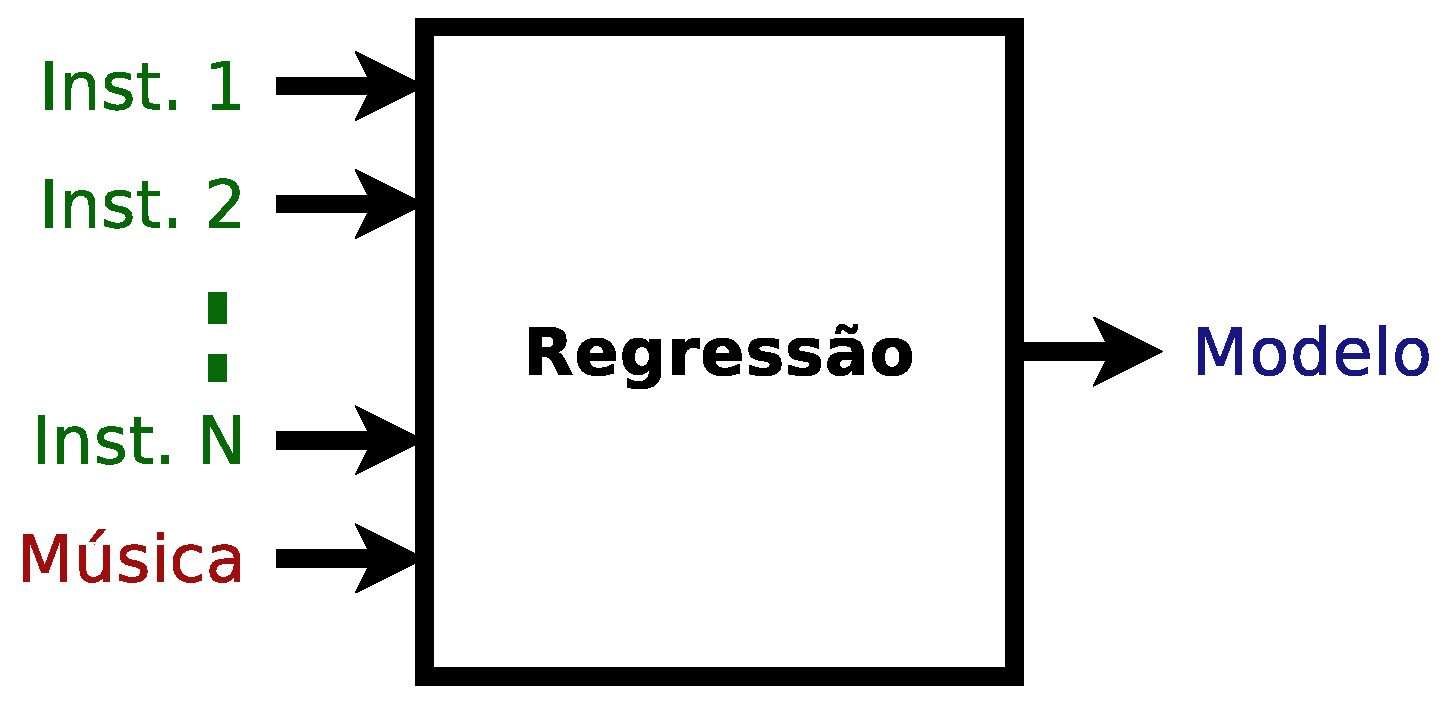
\includegraphics[width=.975\linewidth]{chapters/cap-musicalidade-tecnica/seguindo-instrumentos-1}  
      \caption{Aprendizado supervisionado.}
      \label{fig:seguindo-instrumentos-1}
    \end{subfigure}
    \hfill
    \begin{subfigure}[t]{.45\textwidth}
      \centering
      % include second image
      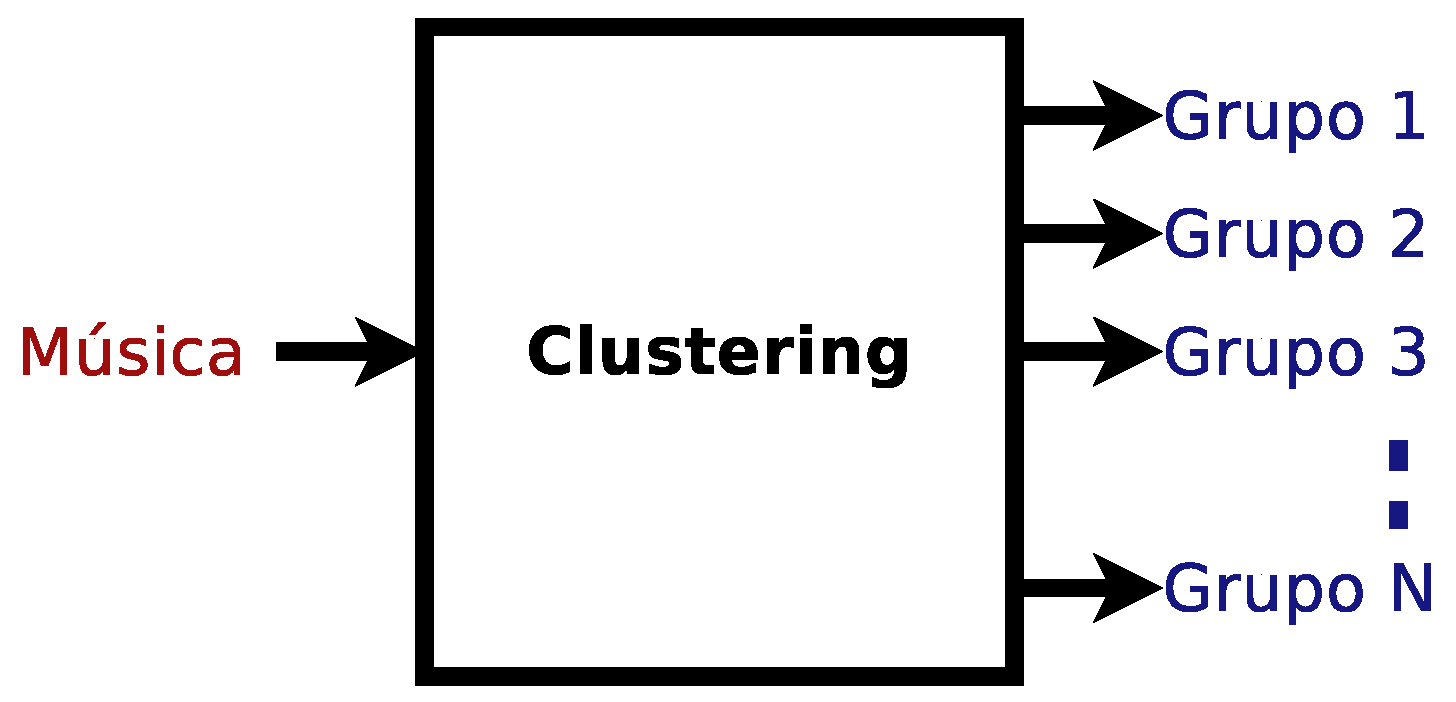
\includegraphics[width=.975\linewidth]{chapters/cap-musicalidade-tecnica/seguindo-instrumentos-2}  
      \caption{Aprendizado não supervisionado.}
      \label{fig:seguindo-instrumentos-2}
    \end{subfigure}
    \caption{Métodos de solução de um problema inverso.}
    \label{fig:seguindo-instrumentos}
\end{figure}



\noindent
\begin{minipage}[b]{0.6\linewidth}
\begin{example}[Brincando com ``puppets'':]
Uma forma de treinar a percepção musical, na detecção isolada de instrumentos, 
é usar um ``puppet'' em cada mão\footnote{Podem ser um par de meias.}.
A ideia principal é colocar uma música e brincar que cada puppet 
mexe a boca seguindo os sons de um instrumento musical específico.
\end{example}
\end{minipage}
\begin{minipage}[b]{0.4\linewidth}
      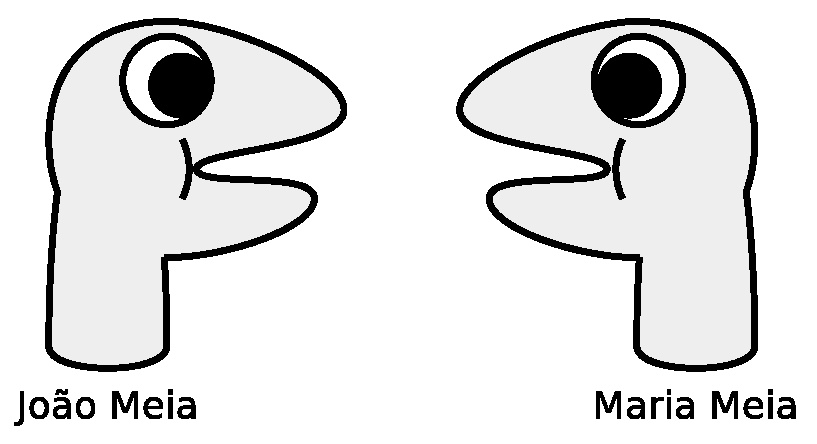
\includegraphics[width=.975\linewidth]{chapters/cap-musicalidade-tecnica/puppets}  
\end{minipage}

\begin{example}[O músico virtual:]
Outra forma de treinar nossa percepção musical é escutar uma música,
escolher algum instrumento executado nela e simular que nos temos um 
instrumento invisível que executamos representando esse instrumento. 
Esta atividade também pode ser realizada em grupo na sala de aula.
\end{example}

\begin{example}[Interpretando os instrumentos:]
Uma vez que consigamos isolar um instrumento da música, 
podemos treinar interpretar-lho corporalmente, para isto podemos
 realizar uma metáfora dos sons com nossos movimentos, 
usando algumas das técnicas já explicadas no livro como: O 
\hyperref[sec:leitmotivdanca]{\textbf{leitmotiv}}, o
\hyperref[sec:mikeymousing]{\textbf{mickey mousing}} ou
a  \hyperref[subsubsec:musicvisualization]{\textbf{visualização musical}}.
\end{example}

\begin{example}[Treinando no choro:]
Quando iniciamos nosso treinamento, 
ter múltiplas camadas de instrumentos pode ser complexo de separar e isolar.
Neste caso é mais recomendável iniciar a treinar com músicas monofônicas ou  homofônicas,
pois estas tem uma única melodia, e geralmente tem só um acompanhamento percussivo e/ou harmônico.
É simples achar versões de \hyperref[subsec:musicchoro]{\textbf{choros}}, 
\hyperref[subsec:musicchoro]{\textbf{chorinhos}} ou 
\hyperref[subsec:musicsambachoro]{\textbf{samba-choros}} gravados seguindo este formato,
assim que eu recomendo iniciar com este tipo de música.
Podemos por exemplo acompanhar a melodia principal esquecendo o ``tic tic tum'',
e em vez disso acompanhar com cada pisada nossa, ou transferência de peso, 
cada \hyperref[sec:figurasmusicais]{\textbf{figura musical}} da melodia. Logo, 
se nossa habilidade o permitir, podemos acompanhar com \hyperref[subsec:fatordinamica]{\textbf{fatores do movimento}}
a informação da melodia que não esteja contida na sua parte rítmica.
\end{example}





%% https://translate.google.com/translate?sl=en&tl=es&u=http%3A%2F%2Fjoymotiondance.com%2Ftexture%2F
%tem a ver com texturas na musica, cada camada é um instruemnto

\begin{elaboracion}{Falácia lógica da falsa dicotomia}
\index{Falácia!Falsa dicotomia}
\index{Falácia!Falsa dilema}
\label{ref:falsadilema}
A falácia lógica da falsa dicotomia também é chamada de falso dilema. 
Esta descreve uma situação em que dois pontos de vista são colocados 
como se fossem as únicas opções que podem ser tomadas, sendo descritas como exclusivas,
quando na verdade existem outras opções ou pontos intermédios a serem considerados
\cite[pp. 163]{rainbolt2012critical}.
\end{elaboracion}


%%%%%%%%%%%%%%%%%%%%%%%%%%%%%%%%%%%%%%%%%%%%%%%%%%%%%%%%%%%%%%%%%%%%%%%%%%%%%%%%
%%%%%%%%%%%%%%%%%%%%%%%%%%%%%%%%%%%%%%%%%%%%%%%%%%%%%%%%%%%%%%%%%%%%%%%%%%%%%%%%
%%%%%%%%%%%%%%%%%%%%%%%%%%%%%%%%%%%%%%%%%%%%%%%%%%%%%%%%%%%%%%%%%%%%%%%%%%%%%%%%
\index{Musicalidade!Ritmo vs. melodia}
\subsection{Falsa dicotomia entre dançar no ritmo e dançar na melodia}
\label{sec:ritmovsmelodia}
Tenho observado que alguns dançarinos descrevem uma marcada separação entre dançar no ritmo e
dançar na melodia; como se, quando estivéssemos fazendo um, não poderíamos fazer u outro;
por outro lado, alguns descrevem que dançar na melodia é dançar com musicalidade e dançar no ritmo não,
ou vice-versa.
Como já foi explicado em seções anteriores, esta percepção dual e exclusiva é
na verdade uma  \hyperref[ref:falsadilema]{\textbf{falsa dicotomia}},
pois como vimos na Pag. \pageref{sec:pos:Melodia} e na Seção \ref{sec:aspectosusicalidade},
a melodia é indivisível do ritmo, 
um ritmo pode ser descrito sem precisar indicar as mudanças de \hyperref[sec:pos:Altura]{\textbf{tom}},
mas não existe uma melodia que possa ser descrita sem indicar o ritmo\footnote{É dizer as mudanças na duração das notas musicais.},
mesmo que esse ritmo seja monótono ou simples demais.
Estendendo esta ideia da música para a dança, uma pessoa, se assim o desejasse, poderia 
dançar seguindo o ritmo sem usar informação das mudanças de tom;
porém, não poderia dançar na melodia sem usar informação do \hyperref[sec:pos:Ritmo]{\textbf{ritmo}}, 
da \hyperref[def:Metrica]{\textbf{métrica}} ou do \hyperref[ref:Pulso]{\textbf{pulso}},
pois a melodia contem todos estes.
\begin{example}[Dançando na textura monofônica:]
\label{ex:ritmovsmelodia}
A Figura \ref{fig:ritmo-melodia-1} mostra dois exemplos nomeados como movimento 1 e 2,
onde um dançarino tem como base musical uma única melodia sem acompanhamento 
(\hyperref[subsec:monofonica]{\textbf{textura monofônica}}).
\begin{itemize}
\item O movimento 1 usa a informação A ($I_{A}$), proveniente da parte rítmica da melodia,
e a informação B ($I_{B}$), proveniente da informação da melodia que não está contida na parte rítmica.
Neste caso a informação $I_A < I_B$, pelo que as pessoas comumente descrevem a este caso como dançar na melodia.  
\item O movimento 2 usa a informação C ($I_{C}$), proveniente da parte rítmica da melodia,
e a informação D ($I_{D}$), proveniente da informação da melodia que não está contida na parte rítmica.
Neste caso a informação $I_C > I_D$, pelo que as pessoas comumente descrevem a este caso como dançar no ritmo.
\end{itemize}
\end{example}

\begin{figure}[!h]
\centering
      % include first image
      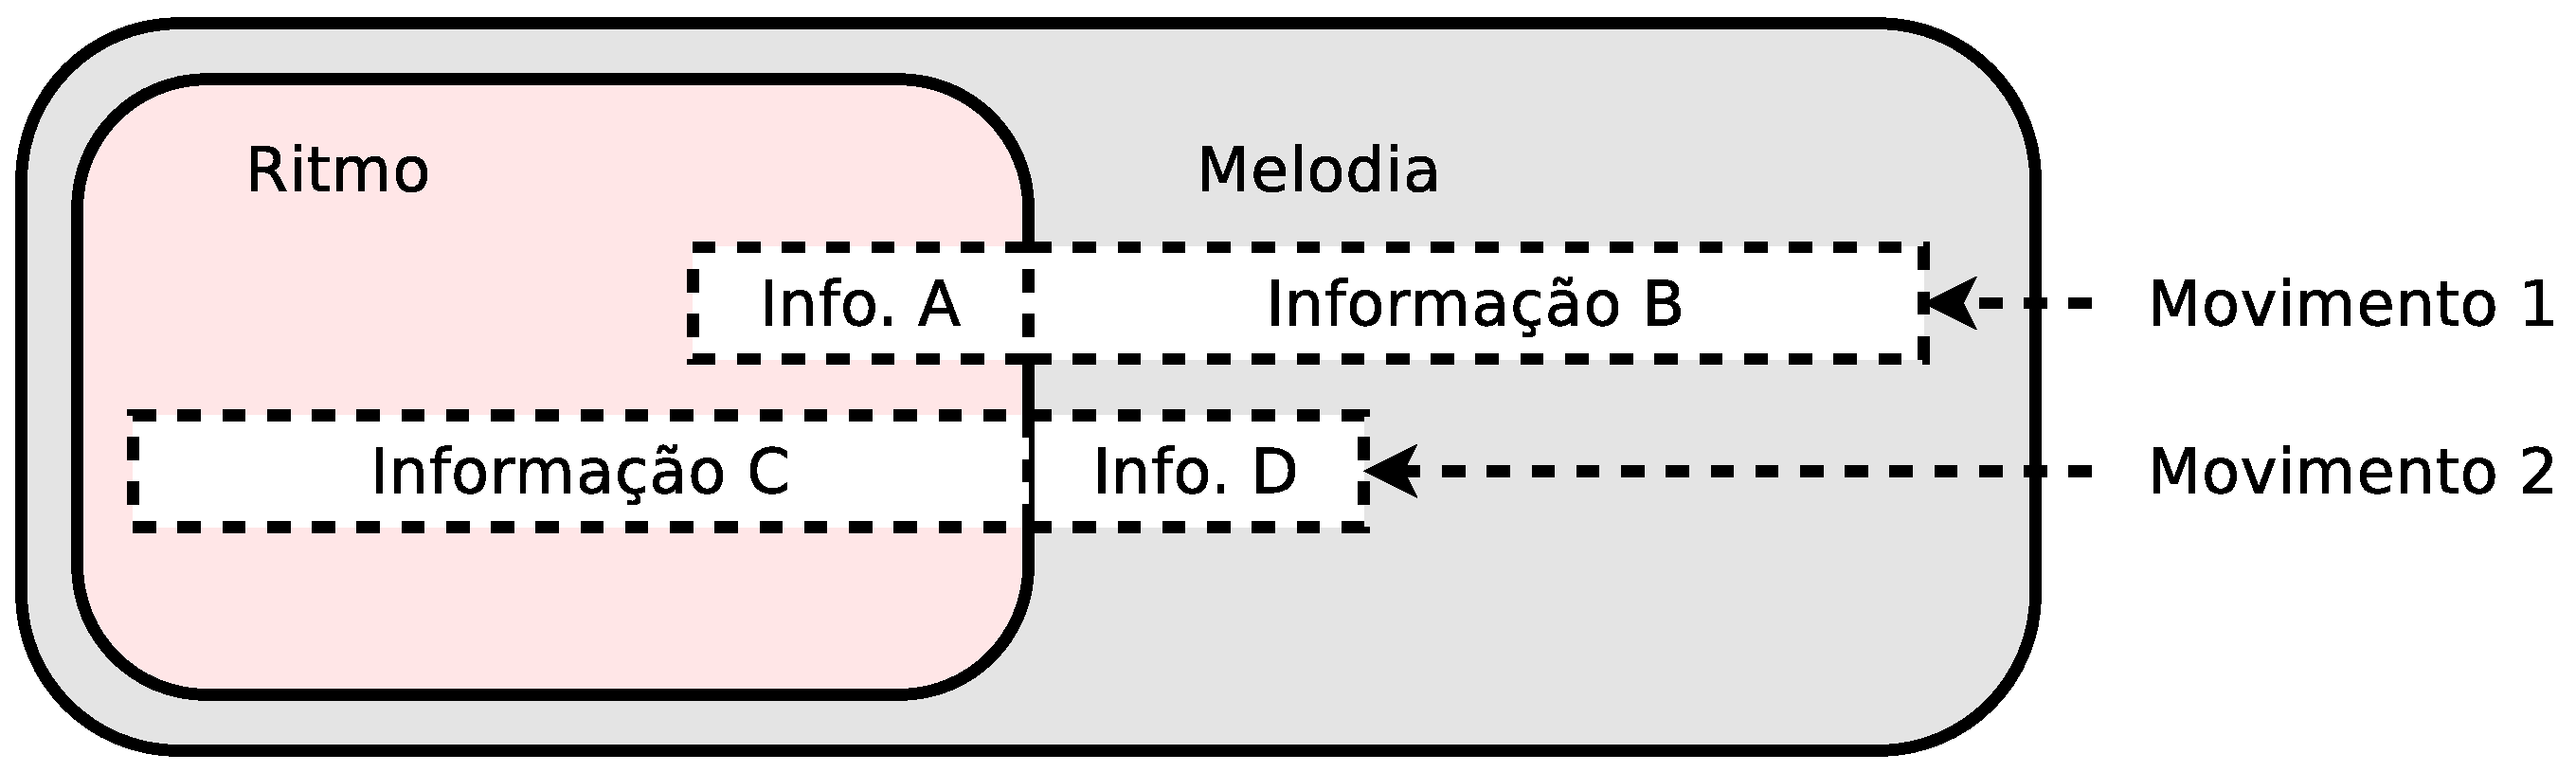
\includegraphics[width=.75\linewidth]{chapters/cap-musicalidade-tecnica/ritmo-melodia-1}  
      \caption{Ritmo e melodia numa música com textura monofônica.}
      \label{fig:ritmo-melodia-1}
\end{figure}
Assim do exemplo anterior observamos que dançar no ritmo e na melodia, não são estados discretos, binários e exclusivos,
e sim descrições continuas e com múltiplas possibilidades, 
que indicam subjetivamente a quantidade de informação que está sendo extraída da parte rítmica\footnote{Do 
acompanhamento percussivo na música ou da parte rítmica da melodia.}
ou da melodia\footnote{De alguma linha melódica principal ou secundaria, ou do acompanhamento harmônico.}
de uma música.

\begin{figure}[!t]
\begin{tcbinformation}{Interpretar a música com o corpo}
Quando dançamos, nosso corpo é incapaz de gerar sons melódicos, só sons rítmicos
mediantes nossas pisadas ou palmas;
por isso o aspecto da musicalidade mais fácil de aplicar é dançar no ritmo,
como se nosso corpo fosse um instrumento mais.

Assim, se observamos cuidadosamente a um dançarino que consideramos que tem musicalidade,
maioritariamente perceberemos que este usa os pés para interpretar a 
\hyperref[def:Metrica]{\textbf{métrica}} e algum ritmo da música\footnote{Em muitas ocasiões 
veremos que um dançarino interpreta de forma literal algum ritmo na música,
pisando uma vez por cada figura musical da voz escolhida, 
aplicando na intensidade de suas pisadas a métrica da música.} mediante alguma técnica como o 
\hyperref[sec:mikeymousing]{\textbf{mickey mousing}} u outra,
e usa o corpo como um todo para interpretar a melodia usando 
\hyperref[subsec:fatordinamica]{\textbf{fatores do movimento}}.
\end{tcbinformation} 
\end{figure}

\begin{example}[Dançando na textura monofônica com acompanhamento percussivo:]
\label{ex:ritmovsmelodia2}
A Figura \ref{fig:ritmo-melodia-2} mostra um exemplo nomeado como movimento 1,
onde um dançarino tem como base musical uma melodia com um acompanhamento percussivo 
(\hyperref[subsec:monofonica]{\textbf{textura monofônica}}).
\begin{itemize}
\item O movimento 1 usa a informação A ($I_{A}$), proveniente do ritmo do acompanhamento percussivo,
e a informação B ($I_{B}$), proveniente da informação da melodia que não está contida na sua parte rítmica.
Neste caso a informação $I_A < I_B$ e é tomada de duas fontes distintas dentro da música, 
 as pessoas comumente descrevem a este caso como dançar na melodia. 
\end{itemize}
\end{example}
\begin{figure}[h!]
\centering
      % include first image
      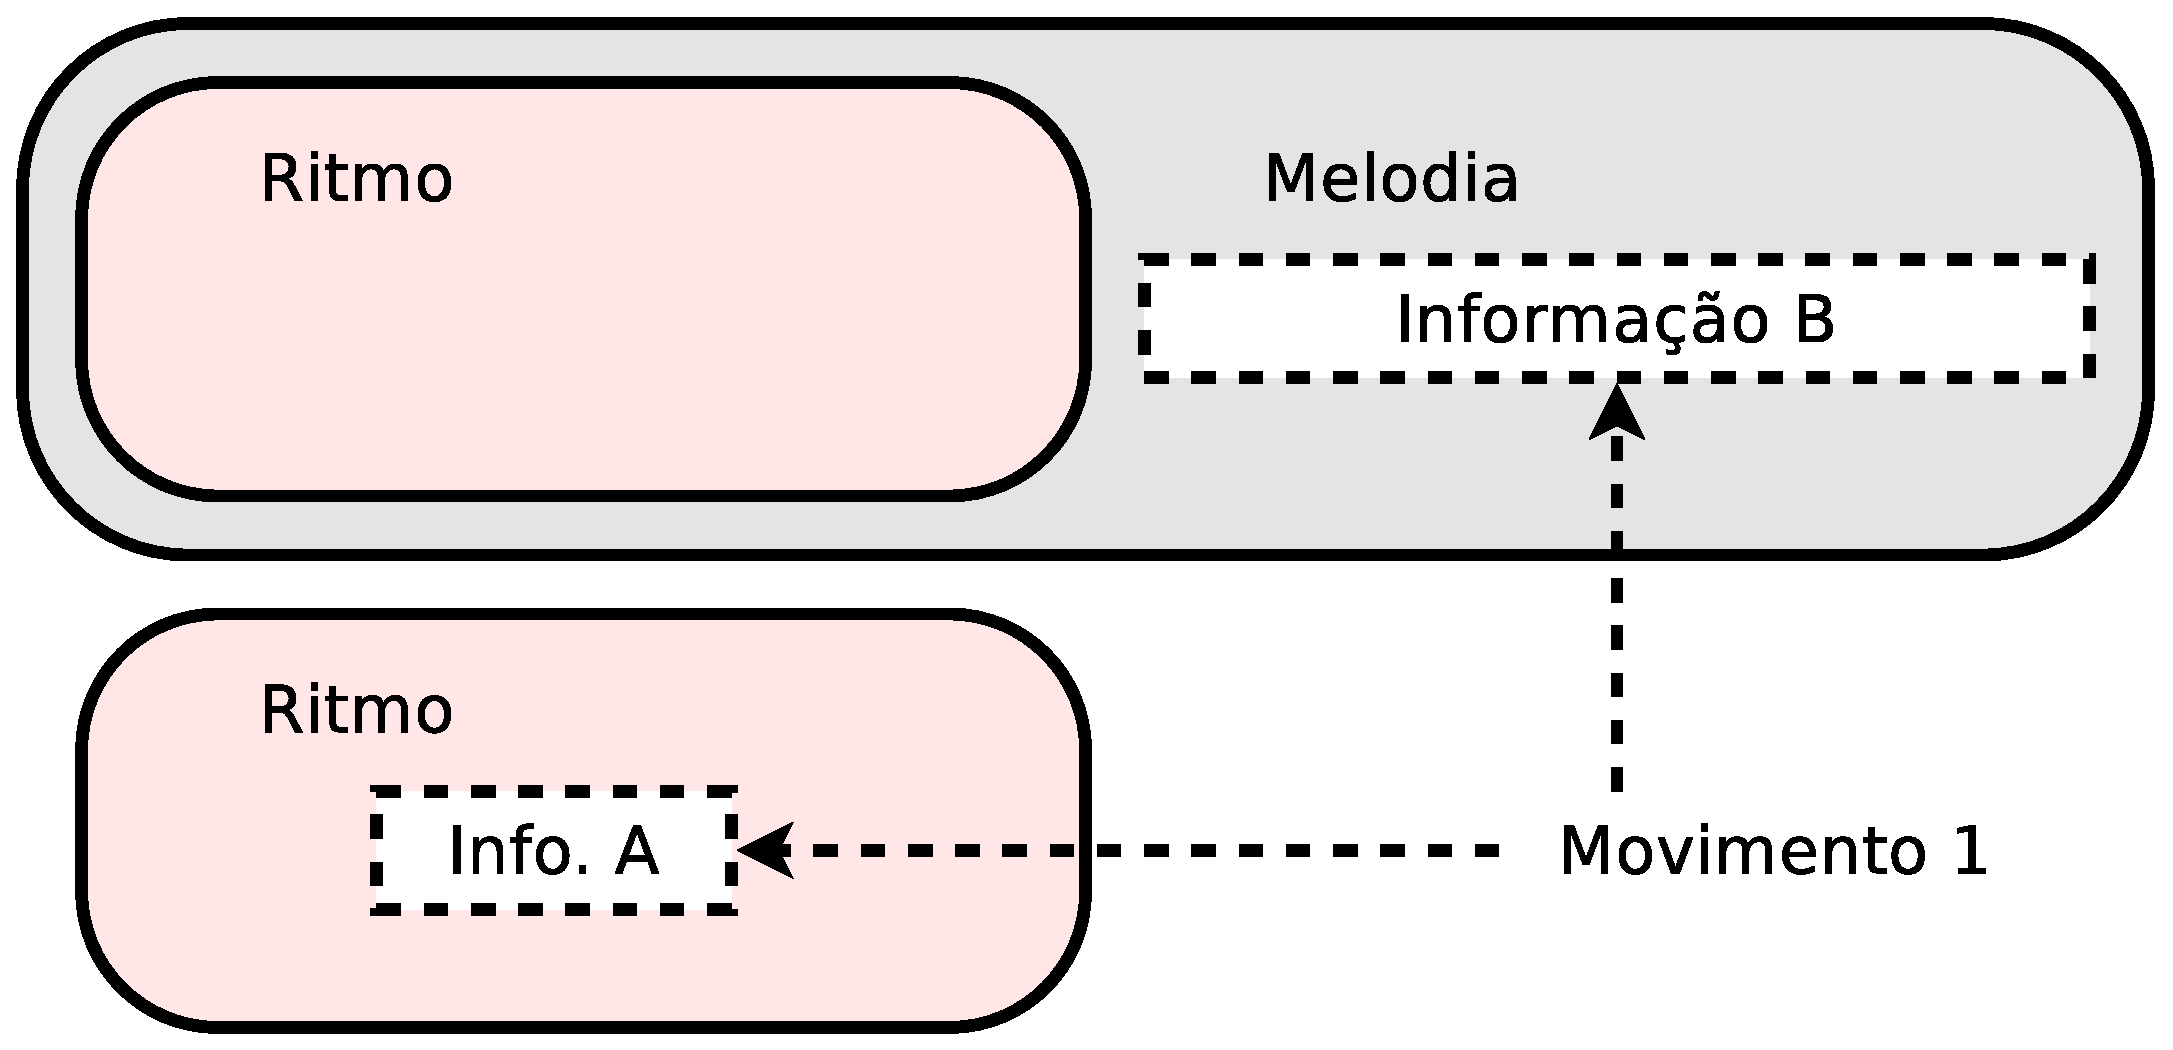
\includegraphics[width=.6\linewidth]{chapters/cap-musicalidade-tecnica/ritmo-melodia-2}  
      \caption{Ritmo e melodia numa música com textura monofônica com acompanhamento percussivo.}
      \label{fig:ritmo-melodia-2}
\end{figure}



Todo o que falamos sobre  \{ritmo, melodia\} é também extensível para 
\{métrica, ritmo\}, \{melodia, música\}, \{métrica, melodia\}, etc.
Pois não existe uma relação de exclusão e sim uma de inclusão;
assim, dependendo do caso, 
escolheremos interpretar mais informação de um âmbito e menos de outro.





%%%%%%%%%%%%%%%%%%%%%%%%%%%%%%%%%%%%%%%%%%%%%%%%%%%%%%%%%%%%%%%%%%%%%%%%%%%%%%%%
%%%%%%%%%%%%%%%%%%%%%%%%%%%%%%%%%%%%%%%%%%%%%%%%%%%%%%%%%%%%%%%%%%%%%%%%%%%%%%%%
%%%%%%%%%%%%%%%%%%%%%%%%%%%%%%%%%%%%%%%%%%%%%%%%%%%%%%%%%%%%%%%%%%%%%%%%%%%%%%%%


\index{Técnica vs. sentimentos-emoções}
\subsection{Falsa dicotomia entre a técnica e os sentimentos-emoções}
\label{subsec:tecnica-sentimentos}
Eu tenho percebido que para muitas pessoas, na dança existe uma relação de exclusão e contraditória 
entre se movimentar seguindo os \hyperref[subsec:filling]{\textbf{sentimentos}} e as 
\hyperref[subsec:emotion]{\textbf{emoções}},
ou fazê-lo seguindo uma técnica. 
De modo que tenho visto pessoas dando pontos de vista a favor ou em contra de alguma destas abordagens.

Na minha opinião existe uma \hyperref[ref:falsadilema]{\textbf{falsa dicotomia}} entre dançar 
seguindo uma técnica e dançar seguindo nossos sentimentos e emoções.
Geralmente as pessoas observam este falso dilema como está representado no mapa mental da
Figura \ref{fig:tecniva-sentimento:a};
onde os símbolos $\bigtriangleup$  representam os movimentos executados com o uso de nossos sentimentos e emoções,
e os símbolos $\Box$ representam os movimentos executados com o uso de técnicas.
\begin{figure}[ht]
\centering
    \begin{subfigure}{.32\textwidth}
      \centering
      % include first image
      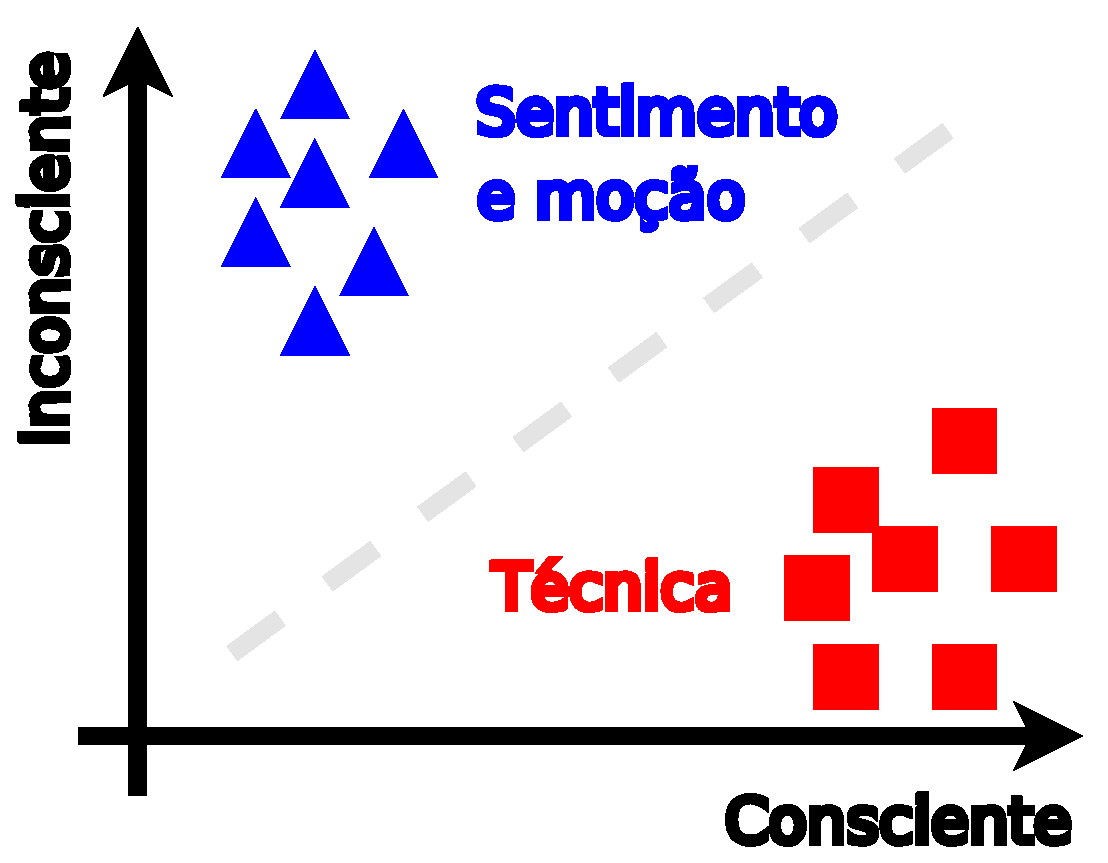
\includegraphics[width=.975\linewidth]{chapters/cap-musicalidade-tecnica/tecnica-emotion-1}  
      \caption{Visão discreta do problema.}
      \label{fig:tecniva-sentimento:a}
    \end{subfigure}
    \hfill
    \begin{subfigure}{.32\textwidth}
      \centering
      % include second image
      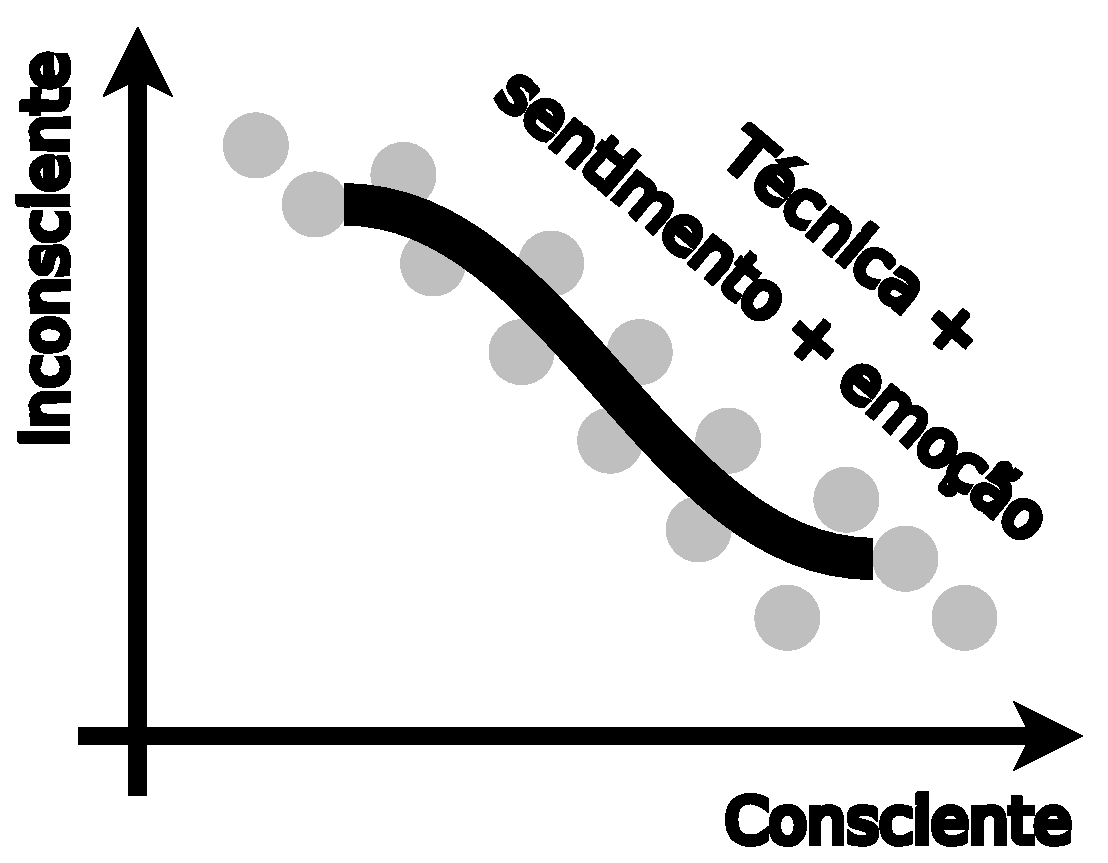
\includegraphics[width=.975\linewidth]{chapters/cap-musicalidade-tecnica/tecnica-emotion-2}  
      \caption{Visão continua do problema.}
      \label{fig:tecniva-sentimento:b}
    \end{subfigure}
    \hfill
    \begin{subfigure}{.32\textwidth}
      \centering
      % include second image
      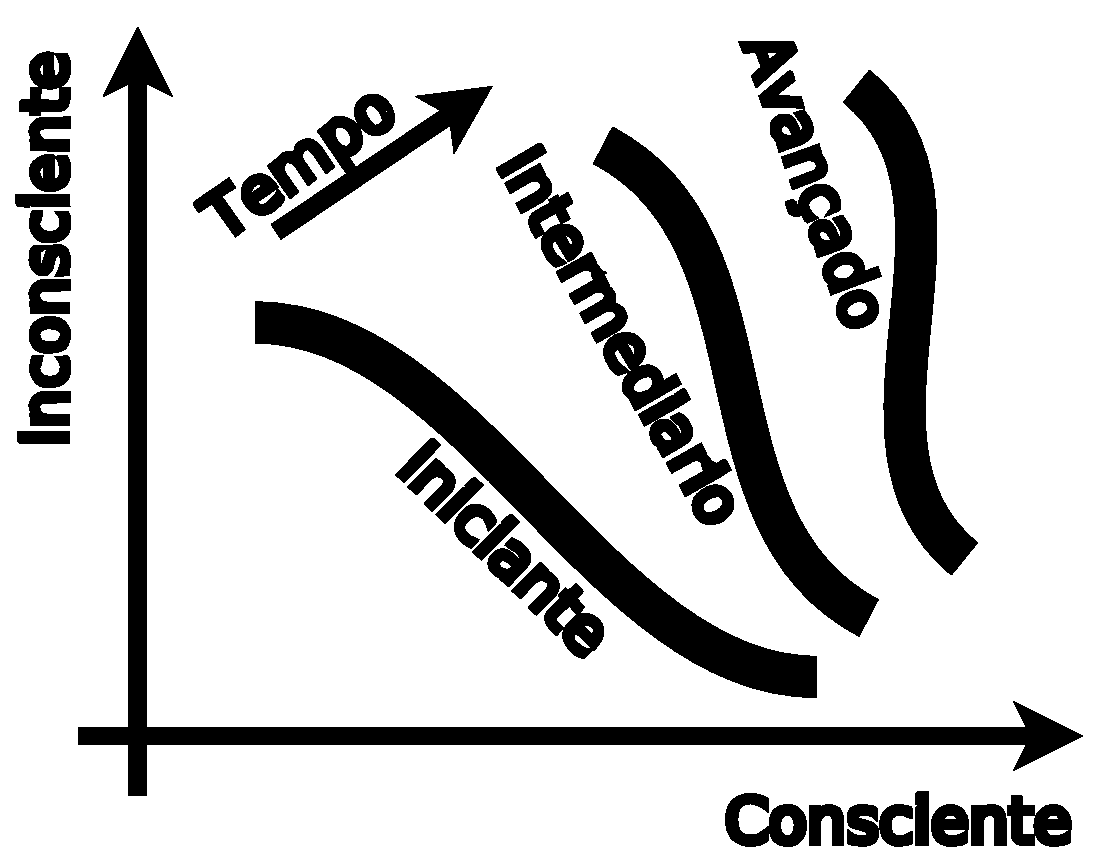
\includegraphics[width=.975\linewidth]{chapters/cap-musicalidade-tecnica/tecnica-emotion-3}  
      \caption{Visão continuo multinível.}
      \label{fig:tecniva-sentimento:c}
    \end{subfigure}
    \caption{Visão subjetiva entre a técnica e os sentimentos-emoções.}
    \label{fig:tecniva-sentimento}
\end{figure}
Como pode ser visto, algumas pessoas tendem a separar estas abordagens em dois grupos bem definidos;
porém, como descreve essa figura, na verdade as pessoas que dançam com técnicas ($\Box$),
o que realmente estão fazendo é dançar com muita consciência do seus movimentos
ou com consciência nas partes mais significativas deste,
e deixando muito pouco ou coisas pouco relevantes a serem executados de forma inconsciente;
por outro lado, as pessoas que dançam seguindo as \hyperref[subsec:emotion]{\textbf{emoções}} e 
\hyperref[subsec:filling]{\textbf{sentimentos}} $\bigtriangleup$,
estão dançando realizando maiormente movimentos escolhidos de forma inconsciente 
e em menor grado movimentos executados de forma consciente.
De modo que não existe em nossos movimentos uma relação binária entre consciência e inconsciência,
e sim muitos pontos intermediários que descrevem de forma continua
todos os tipos de abordagens que podemos seguir na dança.
A Figura \ref{fig:tecniva-sentimento:b} mostra esta ideia num novo mapa mental,
onde nossos movimentos estão representados com o simbolo $\bigcirc$
indicando distintas combinações de consciência e inconsciência.
Para reforçar a ideia de continuidade foi desenhada uma curva que representa as 
distintas possibilidades que podem tomar nossos movimentos na dança.
\begin{example}[Estudante iniciante:] Um estudante de dança, quando recebe
as indicações de um novo movimento ou treinamento, 
executa ele tomando em conta de forma consciente muitos detalhes deste.
Com o tempo esse exercício fica tão interiorizado que vira inconsciente,
e se este estudante não reflete sobre seu próprio processo de aprendizagem, pode chegar a acreditar 
que simplesmente um dia sentiu o que devia sentir e conectou com o trabalho proposto,
quando em verdade ouve um processo de transformação desde o consciente ate o inconsciente.
\end{example}
Mesmo nesse grupo de movimentos que já trabalhamos, 
onde temos distintos níveis de consciência  e inconsciência,
podemos obter melhorias com o tempo e o treino, a Figura \ref{fig:tecniva-sentimento:c} 
mostra um mapa mental mostrando esta característica.
É interessante ressaltar que, como vimos na Seção \ref{sec:atencao}, 
nossa capacidade de \hyperref[sec:atencao]{\textbf{atenção}} 
é bastante limitada, de modo que a quantidade de coisas que podemos fazer de forma consciente 
tem um limite fácil de atingir; porém a quantidade de coisas que podemos fazer em paralelo de 
forma inconsciente é maior.
Assim, como vimos na Seção \ref{sec:aprendizagem}, 
podemos dividir em quatro estágios nosso \hyperref[sec:aprendizagem]{\textbf{processo de aprendizagem}}:
\begin{inparaitem}
\item incompetência inconsciente (II), \item incompetência consciente (IC), 
\item competência consciente (CC) e \item competência inconsciente (CI).
\end{inparaitem}
Sendo que estes dois últimos, CC e CI, 
são os correspondentes mais próximos à técnica e os 
\hyperref[ref:emotionsentimental]{\textbf{sentimentos-emoções}} na dança, respetivamente. 
Porém, como falamos ao principio, este aspecto não é binário e todo movimento 
tem uma parte de técnica e uma parte de sentimento, 
uma parte de consciente e uma parte de inconsciente na sua execução;
a Figura \ref{fig:tecnica-emotion-4} mostra esta característica mediante um mapa mental
que mostra um movimento que consideraríamos executado com técnica e 
outro que consideraríamos executado com sentimento e emoção.
\begin{figure}[ht]
\centering
    \begin{subfigure}[t]{.48\textwidth}
      \centering
      % include first image
      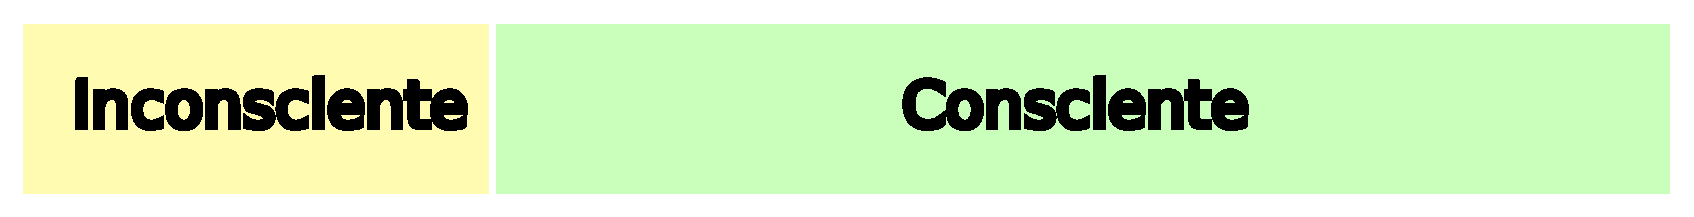
\includegraphics[width=.975\linewidth]{chapters/cap-musicalidade-tecnica/tecnica-emotion-4a}  
      \caption{Movimento executado com técnica.}
      \label{fig:tecnica-emotion-4:a}
    \end{subfigure}
    \hfill
    \begin{subfigure}[t]{.48\textwidth}
      \centering
      % include second image
      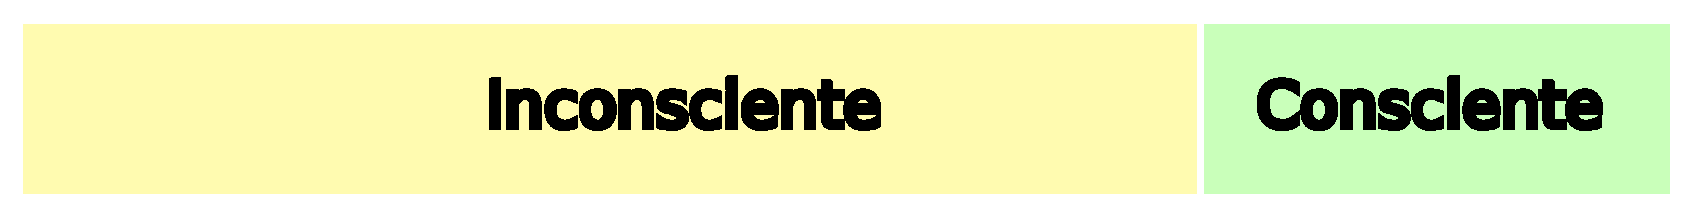
\includegraphics[width=.975\linewidth]{chapters/cap-musicalidade-tecnica/tecnica-emotion-4b}  
      \caption{Movimento executado com sentimento e emoção.}
      \label{fig:tecnica-emotion-4:b}
    \end{subfigure}
    \caption{Estágios mentais na execução dos movimentos.}
    \label{fig:tecnica-emotion-4}
\end{figure}
\begin{description}
\item [Movimentos com técnica:] Quando executamos um movimento mediante o uso da técnica 
comumente as partes mais significativas do movimento são executados de forma consciente.
\item [Movimentos com sentimento-emoção:] Quando executamos um movimento mediante o uso do sentir, 
comumente os movimentos são maiormente executados de forma inconsciente.
\end{description}
Ate agora pode parecer mais interessante que todos nossos movimentos sejam maioritariamente inconscientes,
mas isto é porque estamos observando o problema desde o ponto de vista da jornada de um estudante
que quer praticar a dança, pois como é mostrado na Figura \ref{fig:tecnica-emotion-5:a},
este procura com o passo do tempo obter mais habilidades inconscientes,
pois facilitará seu desenvolvimento na dança.
Porém, desde o ponto de vista de um professor,
como é mostrado na Figura \ref{fig:tecnica-emotion-5:b}, 
o interesse deve ir no caminho contrario,
pois em muitos casos quando chegamos à \hyperref[ref:CompetenciaInconsciente]{\textbf{competência inconsciente}}
tendemos a esquecer os detalhes aprendidos na \hyperref[ref:CompetenciaConsciente]{\textbf{competência consciente}}.
Assim, de nada serve saber fazer e não entender, ou perceber, os detalhes de nossos movimentos,
pois isto impedirá que possamos explicar a nossos estudantes os detalhes que apreendemos 
a dar relevância para nosso perfeicionamento profissional.
Destas reflexões se deriva a frase: ``Saber fazer é diferente de saber ensinar''.
\begin{figure}[ht]
\centering
    \begin{subfigure}{.32\textwidth}
      \centering
      % include first image
      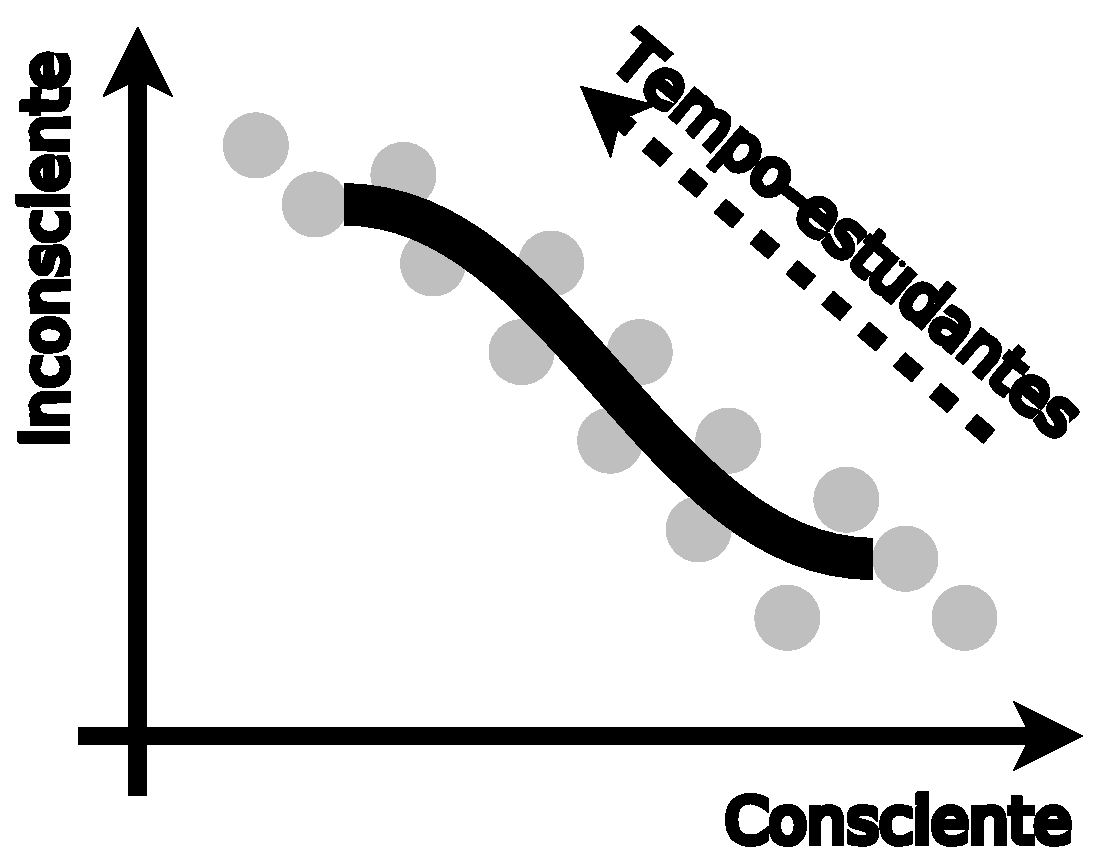
\includegraphics[width=.975\linewidth]{chapters/cap-musicalidade-tecnica/tecnica-emotion-5a}  
      \caption{Sentido de aprendizagem para um estudante.}
      \label{fig:tecnica-emotion-5:a}
    \end{subfigure}
    \qquad
    \begin{subfigure}{.32\textwidth}
      \centering
      % include second image
      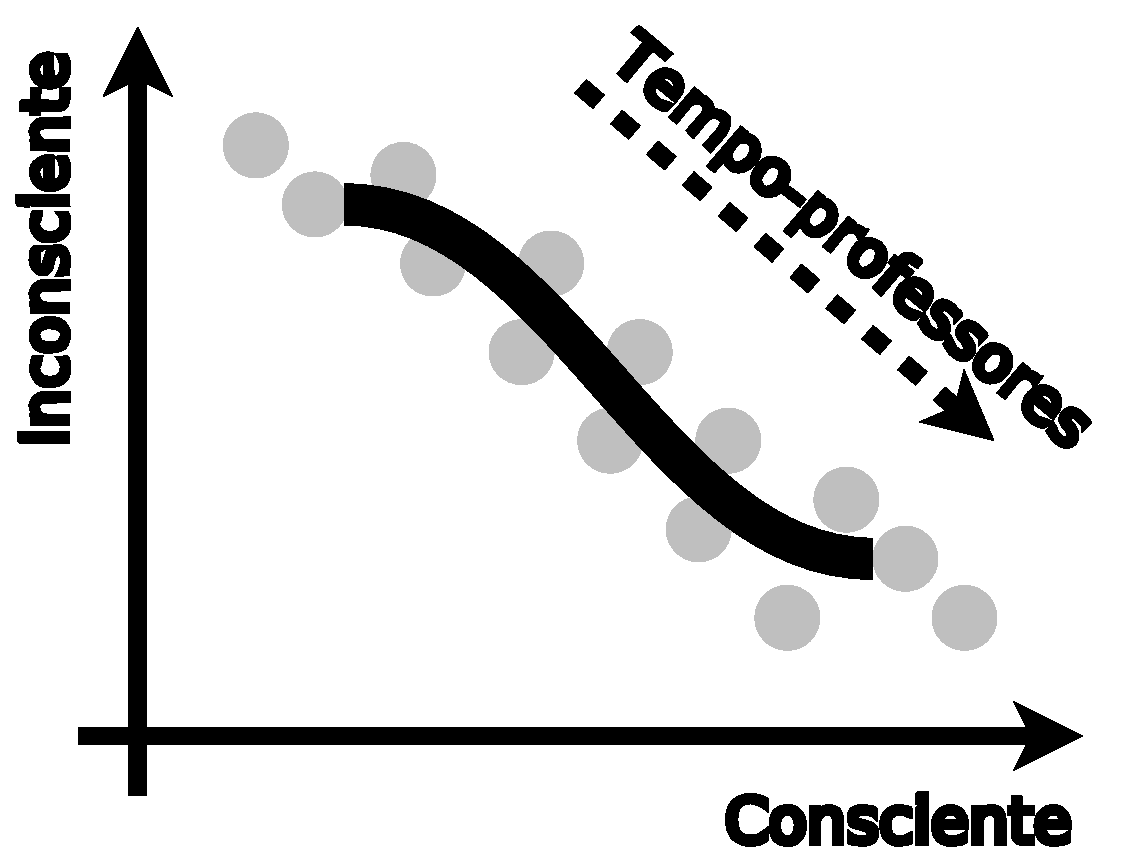
\includegraphics[width=.975\linewidth]{chapters/cap-musicalidade-tecnica/tecnica-emotion-5b}  
      \caption{Sentido de aprendizagem para um professor.}
      \label{fig:tecnica-emotion-5:b}
    \end{subfigure}
    \caption{Fluxo de estudo e autoconhecimento de nossos movimentos.}
    \label{fig:tecnica-emotion-5}
\end{figure}


Tendo em conta isto, se somos professores devemos ter cuidado ao explicar 
um movimento ou exercício a nossos alunos. 
Por exemplo, analisemos o seguinte caso:
\begin{citando}%%
\textbf{O que o professor falou:} Eu senti a música no corpo e 
minhas emoções e sentimentos foram representados na minha dança.\\
\textbf{O que o professor realmente quis dizer:} Eu sei fazer, 
mas não sei exatamente como e porque faço as coisas, 
por isso não sei te explicar como você pode fazer.
\end{citando}
É obvio, como já foi explicado em parágrafos anteriores,
que todo movimento tem uma parte inconsciente e outra consciente,
e que os alunos precisam um mínimo de esperteza corporal (inconsciente) 
para entender algumas decisões e movimentos,
Mas na medida do possível, o professor deve ter um bom nível de autoconhecimento 
para diminuir a brecha de informação no processo formativo do aluno,
e não pretender que eles cheguem por seleção natural da 
\hyperref[ref:IncompetenciaInconsciente]{\textbf{incompetência inconsciente}}
ate a \hyperref[ref:CompetenciaInconsciente]{\textbf{competência inconsciente}}.
A meu modo de ver, uma atitude deste tipo por parte do professor, tentando evitar a parte consciente do trabalho 
e centrando-se principalmente no emocional e sentimental,   
pode ser entendido como uma forma de ``romantizar a ignorância'' 
para evitar aprofundar em aspectos mais técnicos
e de autoconhecimento pessoal.


\index{Aprender passos vs. musicalidade}
\subsection{Falsa dicotomia entre aprender passos e a musicalidade}
\label{ref:pasosvsmusicalidade}
Uma pessoa que conhece várias palavras mas que não tem informação a dizer não pode ser um poeta.
Uma pessoa que tem muita informação a dizer mas que não conhece as palavras ou o idioma também fracassa como poeta. 
No caso da dança, as palavras são nossos passos ou movimentos e a informação 
a extraímos da música, de nosso entorno, de nos mesmos, etc. Assim,
conhecer a música, sua informação e o método para exteriorizar-lha mediante a musicalidade 
não é suficiente para dançar, 
pois precisamos de passos ou movimentos que nos ajudem a expressar-nos e deem identidade ao estilo de dança que escolhemos,
dado que, por exemplo, a linguagem corporal no samba de gafieira é diferente à linguagem no forró ou no tango
e em media estas danças atingem diferentes espectros emocionais.
Assim, precisamos de um \hyperref[sec:BodyControl]{\textbf{controle corporal}} 
bem trabalhado para poder executar os movimentos com precisão em relação ao
quando, o como e onde. 
Precisamos de movimentos ``sinônimos''\footnote{A 
expressão ``movimento sinônimo'' é usada aqui como uma metáfora para indicar um movimento
que pode substituir a outro em objetivo ou na sua função, por exemplo, tendo
a mesma postura de inicio, a postura de fim, o mesmo comprimento em tempo, etc.
de modo que seja possível trocar de movimento para fazer mais variada nossa dança.} 
que nos ajudem a resolver de forma elegante alguma situação na dança.

Em geral existe uma falsa dicotomia entre escolher melhorar nossa dança apontando só a 
um destes fatores, pois é fácil observar mediante a metáfora do poeta,
que o aprimoramento de nossos movimentos é tão importante quanto aprender 
a exteriorizar a informação mediante nossa musicalidade,
o \hyperref[sec:BodyControl]{\textbf{controle corporal}} e
a \hyperref[sec:BodyExpression]{\textbf{expressão corporal}}.  


